\documentclass[10pt]{beamer}
\usetheme[progressbar=frametitle]{metropolis}
\usepackage{appendixnumberbeamer}
\usepackage{booktabs}
\usepackage[scale=2]{ccicons}
\usepackage{pgfplots}
\usepackage{xspace}
\usepackage{mathtools}
\usepackage{amsmath}
\usepackage{amsthm}
\usepackage{amssymb}
\usepackage{latexsym}
\usepackage{subcaption}
\usepackage{hyperref}
\usepackage[ruled]{algorithm2e}
\usepackage{color}
\usepackage{graphicx}
\usepackage{centernot}
\usepackage[cache=false]{minted}
\usepackage[makeroom]{cancel}

\usepackage[style=authoryear,backend=biber]{biblatex}
\addbibresource{docs/bibliography.bib}

\setbeamertemplate{caption}[numbered]
\setbeamersize{description width=2em}
\setbeamertemplate{navigation symbols}{\vspace{-2ex}}

\newcommand{\themename}{\textbf{\textsc{metropolis}}\xspace}
\usepgfplotslibrary{dateplot}
\definecolor{aquamarine}{rgb}{0.5, 1.0, 0.83}
\definecolor{aqua}{rgb}{0.0, 1.0, 1.0}
\definecolor{beige}{rgb}{0.96,0.96,0.86}
\definecolor{lavender}{rgb}{0.87,0.80,1.00}

\setbeamercolor{boxcolor1} {bg=blue, fg=yellow}
\setbeamercolor{boxcolor2} {bg=red, fg=black}
\setbeamercolor{boxcolor3} {bg=cyan, fg=black}

\newcommand{\hlyellow}[1]{\colorbox{yellow}{#1}}
\newcommand{\hlblue}[1]{\colorbox{blue}{#1}}
\newcommand{\hlred}[1]{\colorbox{red}{#1}}

\setminted[python]{
        fontsize=\scriptsize, 
        linenos=true,
        numbersep=6pt,
        gobble=0,
        framesep=0mm,
        bgcolor=lavender} 

\setminted[c]{
        fontsize=\scriptsize, 
        linenos=true,
        numbersep=6pt,
        gobble=0,
        framesep=0mm,
        bgcolor=beige} 

\title{Momentum Transformer Master Class}
\subtitle{Algorithmic Trading Course}
\author{Nick Firoozye}
\date{\today}

\begin{document}
\maketitle



%%%%%%%%%%%%%%%%%%%%
\begin{frame}{Outline}
    \setbeamertemplate{section in toc}[sections numbered]
    \tableofcontents
\end{frame}


%%%%%%%%%%%%%%%%%%%%
% \begin{frame}
%     \begin{figure}
%     \centering
%     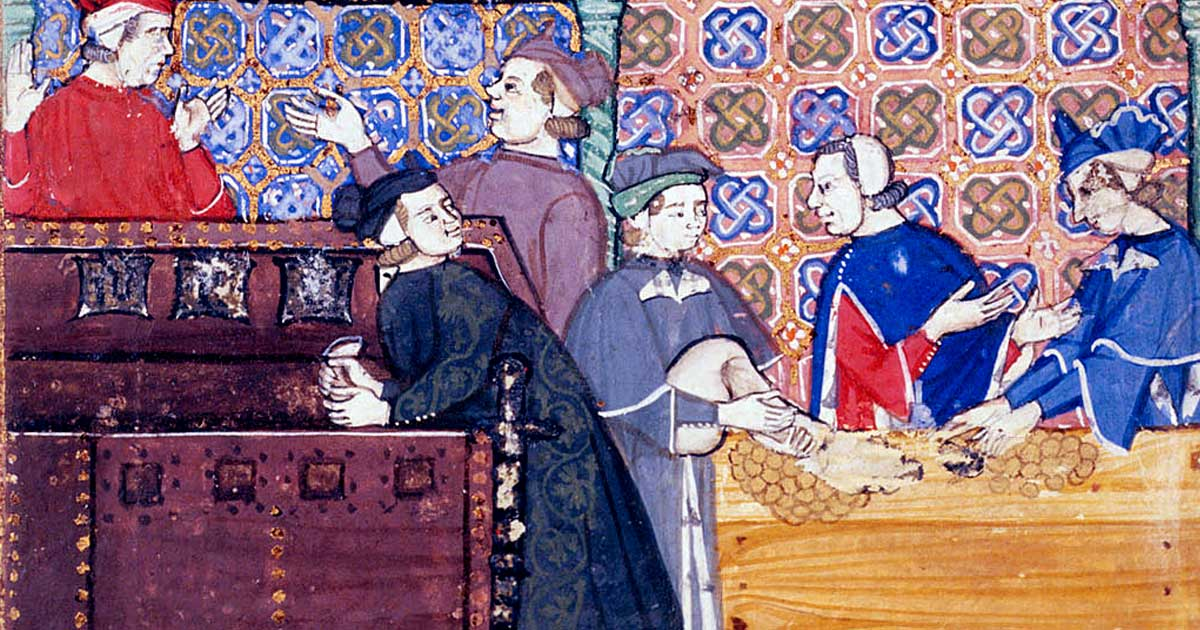
\includegraphics[scale=0.2]{docs/figures/L5/the-birth-of-banking.jpg}
%     \caption{A $14^{th}$ century manuscript depicting bankers in an Italian counting house - Cocharelli - British Library, Cocharelli, Cuttings from a Latin prose treatise on the Seven Vices (avarice) }
%     \label{fig:my_label}
%     \end{figure}
% \end{frame}


% %%%%%%%%%%%%%%%%%%%%

\section{Trend Following Background}
\begin{frame}{Trading Strategies}
    \begin{definition}
        A series of rules that implements buys and sells of a set of assets, given the  information available just prior to the trade.
    \end{definition}
    
    \pause
    \begin{itemize}
    \item 
    {\sl Continuous time} Trading Strategy (with Value $V$) defined by the It\^o Integral:
    
        \begin{align*}
        V(T) = V(\tau) + \int_\tau^T \theta_t\cdot dP_t
        \end{align*} 
        
    where $dP_t\in\mathbf{R}^{k+1}$ a set of price changes, and $\theta_t\in \mathbf{R^{k+1}}$ is the weight-process (conditioned on the filtration 
    ${\cal F}_t$). 
    \pause
    \item 
    In  {\sl discrete time} it is defined as 
    \begin{align*}
        V(t_k) = V(t_0) + \sum_1^k \theta_k\cdot \Delta P_{k+1}
        \end{align*} 
        
    where $\theta_k$ is known at time $t_k$, as is $P_k$ and $\Delta P_{k+1} = P_{k+1} - P_k$. 
    \pause
    % \item 
    % We similarly let $P_t^0$ be the money-market account,   $dP^0_t = r_t\ P^0_t dt$ or  $\Delta P^0_{k+1} = r_k P^0_k$.
    \end{itemize}
\end{frame}


%%%%%%%%%%%%%%%%%%%%
\begin{frame}{Trading Strategies (cont'd)}
    \begin{itemize}
    \item 
    We let $P_t^0$ be the money-market account,   $dP^0_t = r_t\ P^0_t dt$ or  $\Delta P^0_{k+1} = r_k P^0_k$.
    \end{itemize}    
\end{frame}


%%%%%%%%%%%%%%%%%%%%
\begin{frame}{Dynamic Trading Strategies}
    A dynamic strategy is defined as a set of dynamically updated weights, also called the {\em signal} $s_{t-1}$ multiplied by excess returns $r_{t}$, i.e., the strategy returns 
    $$r^s_t = s_{t-1} r_t$$ or, if we track final wealth
    $$W_T = \sum_{t=1}^T r^s_t = \sum_{t=1}^T s_{t-1} r_t$$
    
    The concept of strategy is used frequently in quantitative finance, in particular, {\em self-financing strategies}, see, e.g., Duffie, {\em Dynamic Asset Pricing Theory}, p 83ff.
\end{frame}


%%%%%%%%%%%%%%%%%%%%
\begin{frame}{Example signals}
Strategy weights can be defined in a diverse number of ways, and we will focus on momentum strategies although other strategies may have similarly defined signals. (see, e.g, Firoozye-Koshiyama)
    \begin{itemize}
    \item 
    Simple Moving Average (SMA): 
    
        \begin{align*}
        s_{t-1}=\frac{1}{T}\sum_1^T r_{t-k}
        \end{align*}
    \item 
    Exponentially-Weighted Moving Average (EWMA): 
        
        \begin{align*}
        S_{t-1}=c(\lambda)\sum_{k=1}^\infty \lambda^k r_{t-k}
        \end{align*}
        
    \end{itemize} 
\end{frame}


%%%%%%%%%%%%%%%%%%%%
\begin{frame}{More example signals}
    \begin{itemize}
    \item 
    Difference between current price and moving average
    $$s_{t-1}= p_{t-1} - {1\over T}\sum_1^T p_{t-k}$$
    \item 
    Differences between EWMAs: $$s_{t-1}=c(\lambda_1)\sum \lambda_1^k r_{t-k}-c(\lambda_2)\sum \lambda_2^k r_{t-k}$$
    \item 
    Differences between SMAs: $$s_{t-1}= {1\over {T_1}}\sum_1^{T_1} p_{t-k} - {1\over {T_2}}\sum_1^{T_2} p_{t-j}$$
    \item 
    (with no restriction on the signs of $\phi$'s this may not necessarily be a trend-following strategy) Forecasts from ARMA(p, q) models: $$s_{t-1} = \phi_1 r_{t-1} + \ldots+ \phi_p r_{t-p} + \theta_1 
    \varepsilon_{t-1} + \ldots + \theta_q \varepsilon_{t-q} $$
    \end{itemize}
\end{frame}


%%%%%%%%%%%%%%%%%%%%
\begin{frame}{Final Comments on Signals}

{\bf Note - Convolution kernel:}  All of these strategies can be characterised as $s_{t-1} = \sum_{k=1} \phi_k r_{t-k}$ for some set of weights (or {\em convolution kernel}) $\phi$.

Strategies can also be non-linear functions of any of the above, e.g.,
$$s_t = 1_{\{\sum_1^T r_{T-k}>0\}}-1_{\{\sum_1^T r_{T-k}<0\}}$$
going long one unit whenever the SMA of returns is positive, and short one unit whenever the SMA is negative.

We will focus on the simpler strategies which are linear in historic returns.
\end{frame}


%%%%%%%%%%%%%%%%%%%%
\begin{frame}{Example Strategies}
Standard trading strategies which we will consider in various amounts of detail.
    \begin{itemize}
    \item 
    Buy and hold
    \item 
    Trend-Following - Time-Series
    \item 
    Momentum - Cross-Sectional
    \item 
    Mean-Reversion
    \item 
    Carry
    \item 
    Vol-based strategies (e.g., short-gamma)
    \item 
    Others
    \end{itemize}
\end{frame}


%%%%%%%%%%%%%%%%%%%%
\begin{frame}{Buy-and-Hold}
Buy one unit of asset and hold over horizon.
    \begin{itemize}
    \item  
    Boring!
    \item 
    Only ever meant as a benchmark
    \item 
    If Equities - you are long, so have a positive $\beta$ to the market (usually).
    \item 
    If Bonds - you are long bonds, which often are negatively correlated to Equities.
    \item 
    60-40 Strategy - 60\%  Equities + 40\% bonds is a type of buy-and-hold strategy. Again a benchmark for a global macro fund.
    \end{itemize}
\end{frame}


\section{Trend Following}

%%%%%%%%%%%%%%%%%%%%
\begin{frame}{Trend-Following}
Momentum or Trend Following
    \begin{itemize}
    \item 
    Most widely known Algo style
    \item 
    Ben Graham (the father of {\sl value investing} wrote about it (and invested in it)
    \item 
    Proven to have worked for at least 200 years.
    \end{itemize}
    
    \begin{itemize}
    \item
    Two major forms:
        \begin{itemize}
        \item
        Cross-sectional, i.e., a Momentum factor
        \item
        Time-series, e.g., a CTA
        \end{itemize}
    \item
    Underlies almost all the CTA industry
    \item
    \emph{Not} a diversified source of return
    \item 
    Often thought of as an insurance trade (significant downside protection)
    \end{itemize}
\end{frame}


%%%%%%%%%%%%%%%%%%%%
\begin{frame}{Defining Momentum}
    \begin{definition}[A version of Momentum]
    In it's most basic form: Find a moving average/trend.
        \begin{itemize}
        \item 
        Go Long if 
            \begin{itemize}
            \item 
            Level $>$ Moving average (+threshold)
            \item 
            Short Moving Average $>$ Long Moving Average
            \item 
            Trend is going up
            \item 
            Some combination
            \end{itemize}
        \item Go Short if
            \begin{itemize}
            \item 
            level $<$ Moving average  (- threshold)
            \item 
            Short Moving Average $<$  Long Moving Average
            \item 
            Trend is going down
            \item 
            Some combination
            \end{itemize}
        \end{itemize}
    \end{definition}
\end{frame}


%%%%%%%%%%%%%%%%%%%%
\begin{frame}{Example}
    \begin{figure}
    \centering
    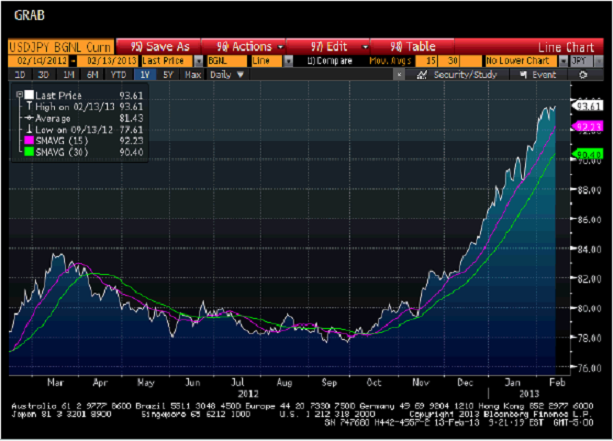
\includegraphics[scale=0.65]{docs/figures/L5/Momentum_JPY.png}
    \caption{USD-JPY and 15/30-day Moving Averages}
    \label{fig:enter-label5}
    \end{figure}
\end{frame}


%%%%%%%%%%%%%%%%%%%%
\begin{frame}{Questions}
    \begin{itemize}
    \item
    How do we establish trend?
    \item
    How far do we look back?
    \item
    Do we normalize signal?
    \item
    Do we cap and floor?
    \item 
    Do we take other nonlinear transformations?
    \end{itemize}
\end{frame}


%%%%%%%%%%%%%%%%%%%%
\begin{frame}{200 Years of Trend Following}
    \begin{figure}
    \centering
    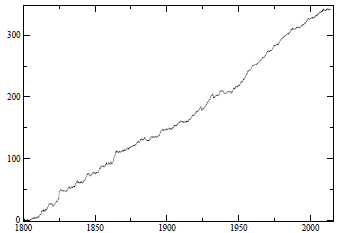
\includegraphics[scale=0.5]{docs/figures/L5/Trend_Following_200y.png}
    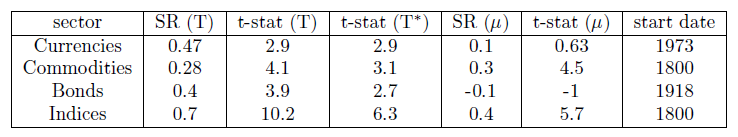
\includegraphics[scale=0.5]{docs/figures/L5/Trend_Following_200y_table.png}
    \caption{Caption}
    \label{fig:enter-label6}
    \end{figure}

Combined Sharpe Ratio of 0.72. \\
Lemp\'eri\`ere et al ‐ {\sl Two Centuries of Trend Following} (2014)
\end{frame}


%%%%%%%%%%%%%%%%%%%%

%%%%%%%%%%%%%%%%%%%%
\begin{frame}{Momentum Factoids}
\begin{alertblock}{Momentum's desirable properties}
    \begin{itemize}
    \item 
    It tends to perform when vol is high. (counter: when vol is low it tends to underperform)
    \item 
    It tends to have positively skewed returns (i.e., it may not win often, but when it wins, it wins big)
    \item 
    The skewness of returns appears greater when measured over longer horizons (e.g., when investors look at quarterly returns they are very highly skewed, compared to daily returns).
    \item 
    Its payoff is similar to that of a straddle, at least empirically. (Fung-Hsieh analysed \href{https://people.duke.edu/~dah7/RFS2001.pdf}{this} despite it being a heuristic )
    \item Makes money in trending markets, including down-trends (insurance)
    \item Loses money in sideways markets (pays for insurance)
    \end{itemize}
    
    We investigate the skewness over different horizons and We also investigate responsiveness to changes in trend.
    \end{alertblock}
\end{frame}





% \section{Momentum and responsiveness}

\section{Momentum and Skewness}



% ---


% ####  Momentum Factoids

% \item See Readings in Appendix for more detail
% \item Returns are (hopefully) positive, with decent Sharpes<!-- .element: class="fragment" data-fragment-index="1" -->
% \item Number of winning trades may be <  50%<!-- .element: class="fragment" data-fragment-index="2" -->
% \item Skewness<!-- .element: class="fragment" data-fragment-index="3" -->
%     \item Returns are positively skewed instantaneously<!-- .element: class="fragment" data-fragment-index="4" -->
%     \item Returns can be more positively skewed over long horizons<!-- .element: class="fragment" data-fragment-index="5" -->
%         \item Skewness peak horizon ~ lookback for EWMA<!-- .element: class="fragment" data-fragment-index="6" -->
%         \item Longer lookbacks = higher and later peaks<!-- .element: class="fragment" data-fragment-index="7" -->
%         \item Shorter lookbacks = earlier peaks<!-- .element: class="fragment" data-fragment-index="8" -->
%         \item Multiple EWMAs = higher peaks, less tapering<!-- .element: class="fragment" data-fragment-index="9" -->
%     \item Winsorizing (caps/floors) damages skewness <!-- .element: class="fragment" data-fragment-index="10" -->
%     \item Winsorizing may be necessary anyway<!-- .element: class="fragment" data-fragment-index="10" -->





%


%%%%%%%%%%%%%55
\begin{frame}{Skewness Analysis}

% #### Martin-Zou
\begin{alertblock}{Skewness - Martin\& Zou}
    \begin{itemize}
        \item  Let returns be  $X_t\thicksim \mathcal{ N}(0,1)$ IID
        \item We can still have a filter with nice properties
       \item Strategy returns $R_t = s_{t-1}X_t$ where $s_{t-1}$ is signal
       \item Consider horizon $T$ returns, i.e., $R_{t+T}=\sum_{\tau=t}^T s_{\tau-1}X_\tau$
       \item We consider EWMA signals 
       \begin{align*}
       s_{t}&=\sum_{k=1}^\infty a_k X_{t-k}\\
       &=c\sum_{k=1}^\infty\rho^k X_{t-k}
        \end{align*}

        where $c$ is a normalizing constant
    \end{itemize}

\end{alertblock}
\end{frame}

\begin{frame}{Calculating Skewness }
\begin{alertblock}{Calculating Skewness}
    
    \begin{itemize}
    \item  We can take first three moments. Skewness is interesting
    \item Let innovation $X_t$ be iid, with zero mean and 3rd moment and unit variance: 
    \begin{itemize}
        \item $\langle X_t,X_s \rangle =0 $  for $t\neq s$
        \item $\langle X_t \rangle=0$, $\langle X_t^2 \rangle =1 $ and $< X_t^3 >=0 $ 
    \end{itemize}
    \item  Zero mean and skewness
     \item Algebra alone will get that:
     \begin{itemize}
        \item Mean: 
        \begin{itemize}
            \item $ < R_{t+T} >= 0 $
        \end{itemize}
        
        \item Variance: 
        \begin{align*}
            \langle R_{t+T}^2 \rangle& = \langle (s_0 X_1+ s_1 X_2+\cdots+ s_{T-1}X_T)^2 \rangle\\
            &= T\sum s_i^2 \langle X_{i+1}^2\rangle \\
            & = T\times\langle s^2\rangle
        \end{align*}
        \end{itemize}
    \end{itemize}
\end{alertblock}
\end{frame}


\begin{frame}{Skewness II}
    \begin{alertblock}{Skewness}
    \begin{itemize}
        \item $ 3^{rd}$ Moment - Skewness:  
        \begin{align*}
        \langle R_{0+T}^3 \rangle & = \langle (s_0 X_1+ s_1 X_2+\cdots+ s_{T-1}X_T)^3 \rangle&\\
        &= \hbox{const} * \cancelto{0}{\langle s_{n_1}  X_{n_1+1} s_{n_2} X_{n_2+1}s_{n_3} X_{n_3+1}\rangle} &\hbox{~with~} n_1<n_2<n_3\\
        & +\hbox{const}*\cancelto{0}{\langle s_n^2 X_{n+1}^2 s_m X_{m+1}\rangle} &\hbox{~with~} n<m\\
        &+ \hbox{const}*\cancelto{0}{\langle s_n^3X_{n+1}^3\rangle}  &\hbox{with~} n>0\\
        & +\hbox{const}* \langle s_n^2 X_{n+1}^2 s_m X_{m+1}\rangle &\hbox{~with~} n>m\\
        &= 3\sum_{0\leq n <  m <T} \langle s_m^2 s_n X_{n+1}\rangle 
        \end{align*}
    \end{itemize}
    Since $s_n^2$ may depend on $X_{m+1}$
\end{alertblock}
\end{frame}


\begin{frame}{Skewness by Horizon}
\begin{alertblock}{Skewness by horizon}
\begin{figure}
    \centering
    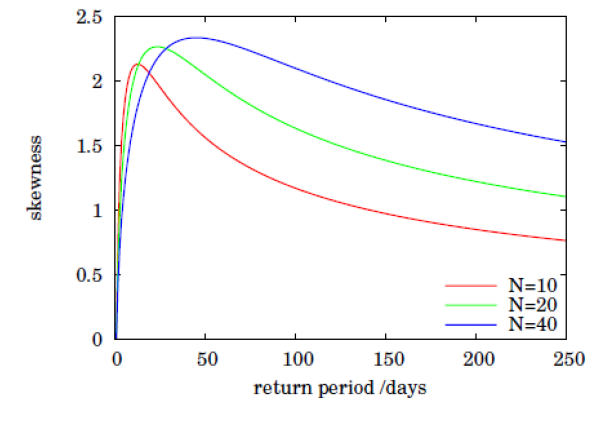
\includegraphics[width=0.5\textwidth]{docs/figures/L5/MartinsSkewnessEWMA1.png}
    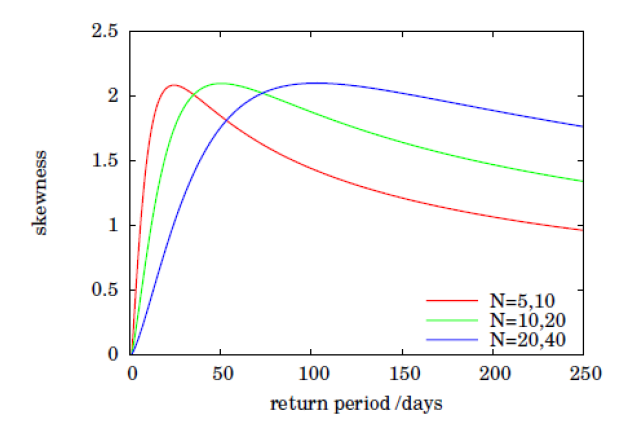
\includegraphics[width=0.5\textwidth]{docs/figures/L5/MartinsSkewnessEWMA2.png}
    
    \caption{Skewness for various horizons \href{https://www.risk.net/derivatives/structured-products/2194247/momentum-trading-skews-me}{Martins-Zou:Momentum Trading:Skews Me}}
    \label{fig:enter-label7}
\end{figure}
\end{alertblock}
\end{frame}


\begin{frame}{Skewness III}
    \begin{alertblock}{Skewness}
    Now if $X_k$ have a non-zero acf:
    \begin{itemize}

 \item Letting signal $$s_k = \sum_{j=0}^\infty a_j X_{k-j}$$ where $a_j$ are fixed filter weights (e.g., $a_j=c\times\rho^j$ for EWMA)
 \item The third moment becomes $$6\sum_1^T(T-j)a_j \gamma_k(a)$$
 \item where $\gamma_k$ is the autocovariance function of weights $a$ i.e., $$\gamma_k^a=\sum_j a_j a_{j+k}$$
\end{itemize}

\end{alertblock}
\end{frame}

% ----




\begin{frame}{Fascinating skewness}

\begin{alertblock}

Why is skewness so interesting?   
\begin{itemize}
    \item  Even an un-skewed return distribution can lead to positive skewness  
    \item (Almost all) risk-averse investors prefer:
    \begin{itemize}
        \item  more positive returns
        \item  less volatility
        \item more positive skewness
     \end{itemize}

\item Why is skewness so strange? 
\begin{itemize}
    \item Interaction between  future signal (at time $T+k$) involving terms from $T$ to $T+k-1$
    \item Interaction between future returns (at times $T$ to $T+k-1$)
\end{itemize}

\item  In reality mean, standard deviation and Sharpe also (even more) interesting!

\end{itemize}

\end{alertblock}
\end{frame}


\begin{frame}{Skewness and Risk Premia}
\begin{alertblock}{Negatively Skewed have higher SR except for Momentum}
\begin{figure}
    \centering
    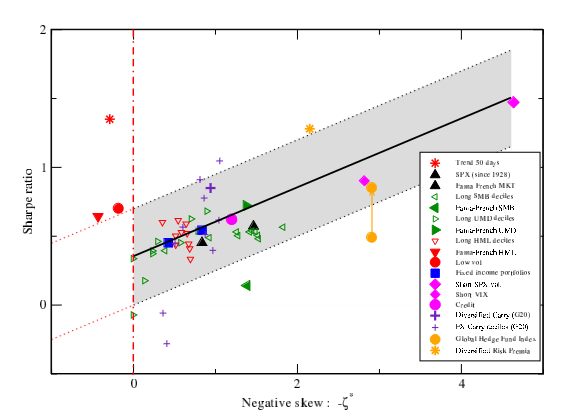
\includegraphics[scale=0.43]{docs/figures/L5/Skew vs Sharpe.png}
    \caption{More negatively skewed have higher Sharpe Ratio. Source: \href{https://arxiv.org/abs/1409.7720}{Lemperiere et al, Risk Premia: Asymmetric Tail Risks and Excess Returns}}
    \label{fig:enter-label8}
\end{figure}
    
\end{alertblock}
    
\end{frame}



\begin{frame} {Trend Following Practicalities }
\begin{alertblock}{Many different methods all lead  to reasonable trend-following strategies}
\begin{itemize}
    \item SMA, EWMA, combinations of signals (crossing EWMA, weighted EWMAs)
    \item Capped and floored signals  ({\sl Winsorising}) 
    \item State-space models (local level and local slope models), etc.  
    \item Loess, or local regressions 
    \item ARIMA models
    \item Wavelets, Fourier decomposition
\end{itemize}

\end{alertblock}
\end{frame}


\begin{frame}{Taxonomy of filtering methods}
    
\begin{alertblock}{Filtering returns}
\begin{itemize}  
    \item Exponentially weighted moving averages (EWMA)
    \item Simple moving averages (SMA)
    \item Normalizing 
    \item Winsorising
    \item Indicator Functions
    \item Combining Signals (Ensemble Methods)
    \item Nonlinear Transforms used as well
\end{itemize}
\end{alertblock}
\end{frame} 

\begin{frame}{Taxonomy II}
\begin{alertblock}{Filtering Levels (Differences of levels)}
\begin{itemize}

    \item Level vs EWMA
    \item Level vs SMA
    \item Crossing moving averages (specific order indicating momentum)
    \begin{itemize}

        \item e.g., $\langle y\rangle_5 >\langle y\rangle_{10}>  \langle y\rangle_{30}$ go very long,
        \item $\langle y\rangle_5 < \langle y\rangle_{10} < \langle y\rangle_{30}$ go very short.
        \item Sum or various horizon indicator functions of levels
        
    \end{itemize}        
    \item Differences of filters
    \item Holt-Winters (H-W) and local  trend extraction
\end{itemize}    

\end{alertblock}
In spite of wide variety of models, momentum returns are almost identical \href{http://papers.ssrn.com/sol3/papers.cfm?abstract_id=2603731}{Levine and Pedersen, Which trend is your friend?}
\end{frame}



% \item Kalman Filter
%     \item Local Level model (covered in MR section) is  asymptotically the same as EWMA<!-- .element: class="fragment highlight-current-blue"  data-fragment-index="1" -->
%     \item Local trend model (covered in MR section) is  asymptotically the same  as H-W<!-- .element: class="fragment highlight-current-blue"  data-fragment-index="2" -->
%     \item Allow for breaks, piecewise constant or piecewise linear trends<!-- .element: class="fragment highlight-current-blue"  data-fragment-index="3" -->


% \item Loess
%     \item Localised Regressions<!-- .element: class="fragment highlight-current-blue"  data-fragment-index="1" -->
%     \item Backwards looking windows (e.g., exponentially weighted)<!-- .element: class="fragment highlight-current-blue"  data-fragment-index="2" -->
%     \item Similarities to Holt-Winters<!-- .element: class="fragment highlight-current-blue"  data-fragment-index="3" -->
% \item <!-- .element: class="fragment highlight-current-blue"  data-fragment-index="4" -->ARIMA
%     \item Wide variety of available model forms<!-- .element: class="fragment highlight-current-blue"  data-fragment-index="5" -->
%     \item Forecasts can be erratic unless OOS testing<!-- .element: class="fragment highlight-current-blue"  data-fragment-index="6" -->
%     \item ARIMA(0,1,1) is EWMA<!-- .element: class="fragment highlight-current-blue"  data-fragment-index="7" -->
%     \item ARIMA(0,2,2) is Holt-Winters<!-- .element: class="fragment highlight-current-blue"  data-fragment-index="8" -->

% \item 





%%%%%%%%%%%%%%%%%%%%
\begin{frame}{Skewness in Practice}
\textsf{Now, despite the fact that the time series of returns is here assumed to be a sequence of iid variables following a normal distribution, the strategy returns $r_{t+T}^{s}$ time series has different properties, in particular it displays skewness, i.e. trend followers lose more often than they gain, as shown in a paper by Bouchaud and Potters (2005). }

    \begin{figure}
        \centering
        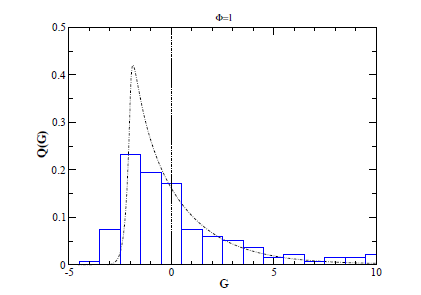
\includegraphics[scale=0.45]{docs/figures/L5/chf_usd_skew.png}
        \caption{Caption}
        \label{fig:enter-label9}
    \end{figure}
\end{frame}


\begin{frame}{Skewness and Nonlinear Transforms}
\begin{figure}
    \centering
    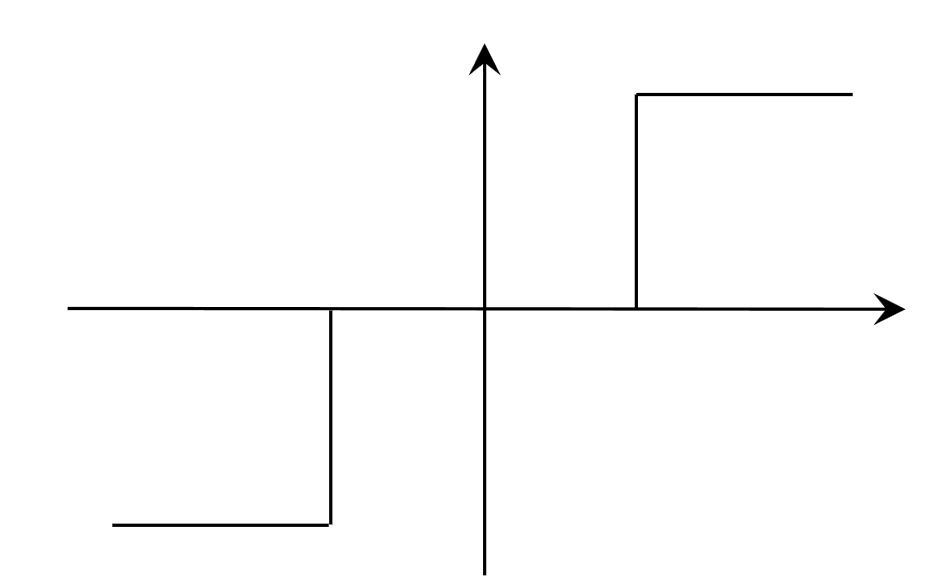
\includegraphics[scale=0.2]{docs/figures/L5/step_function.png}
    \caption{Step Function}
    \label{fig:enter-label123}
\end{figure}

\end{frame}

\begin{frame}{Skewness and Nonlinear Transforms}
\begin{figure}
    \centering
    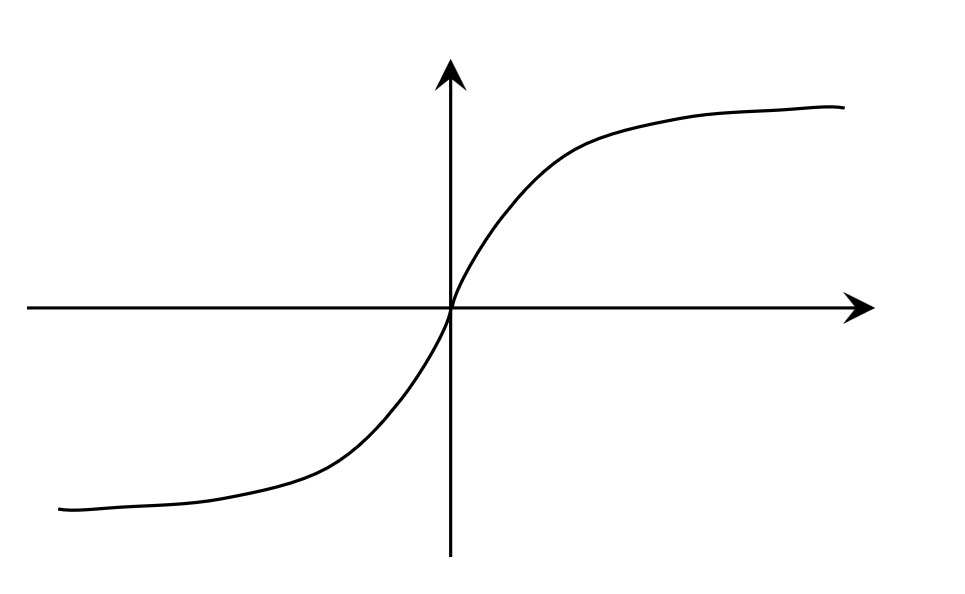
\includegraphics[scale=0.2]{docs/figures/L5/sigmoid.png}
    \caption{Sigmoid}
    \label{fig:enter-label111}
\end{figure}

\end{frame}

\begin{frame}{Skewness and Nonlinear Transforms}
\begin{figure}
    \centering
    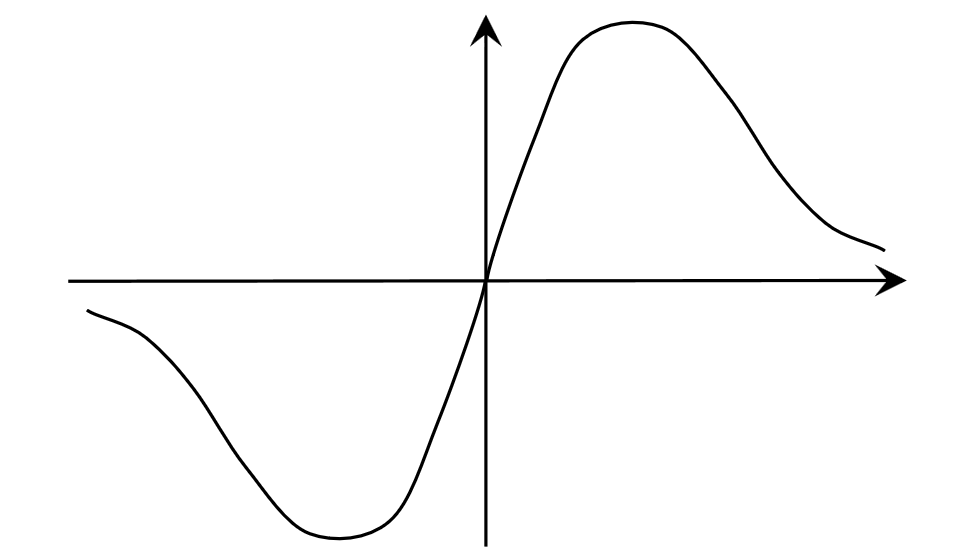
\includegraphics[scale=0.2]{docs/figures/L5/reverse_sigmoid.png}
    \caption{Reverse Sigmoid}
    \label{fig:enter-label110}
\end{figure}

\end{frame}

\begin{frame}{Skewness and Nonlinear Transforms}
\begin{figure}
    \centering
    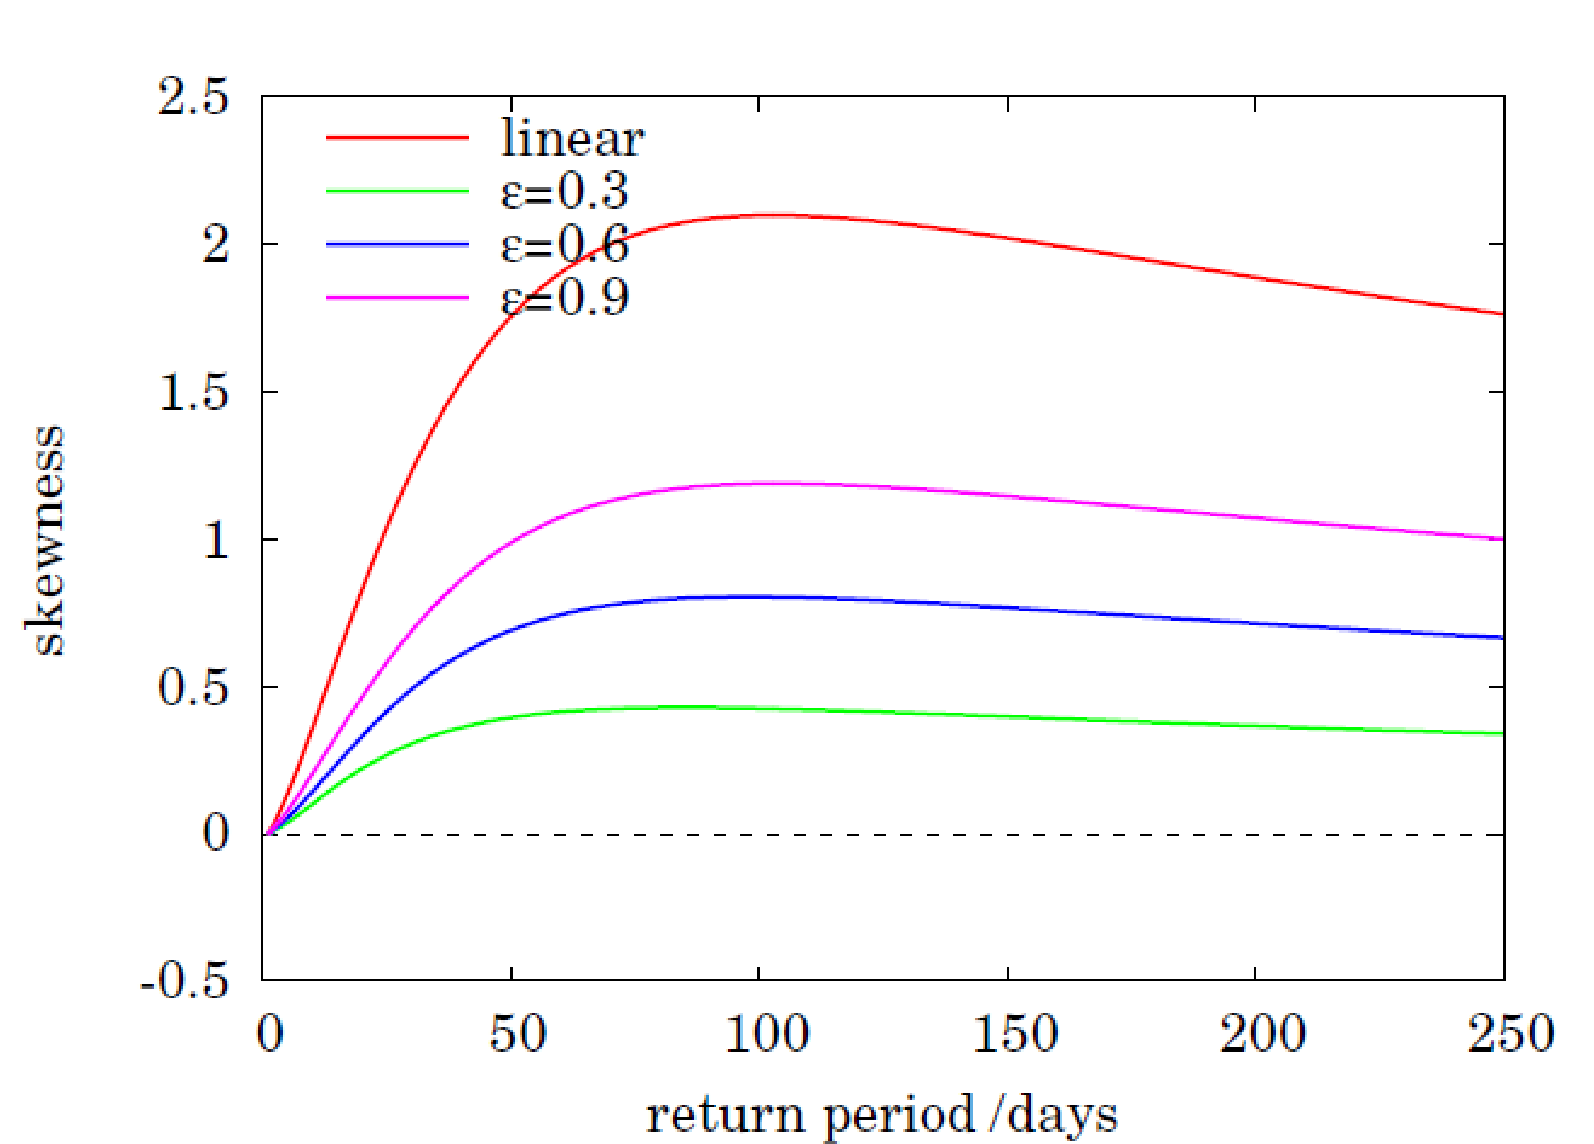
\includegraphics[scale=0.15]{docs/figures/L5/step_skewness.png}
    \caption{Step Skewness - threshold lowers it}
    \label{fig:enter-label2}
\end{figure}

\end{frame}

\begin{frame}{Skewness and Nonlinear Transforms}
\begin{figure}
    \centering
    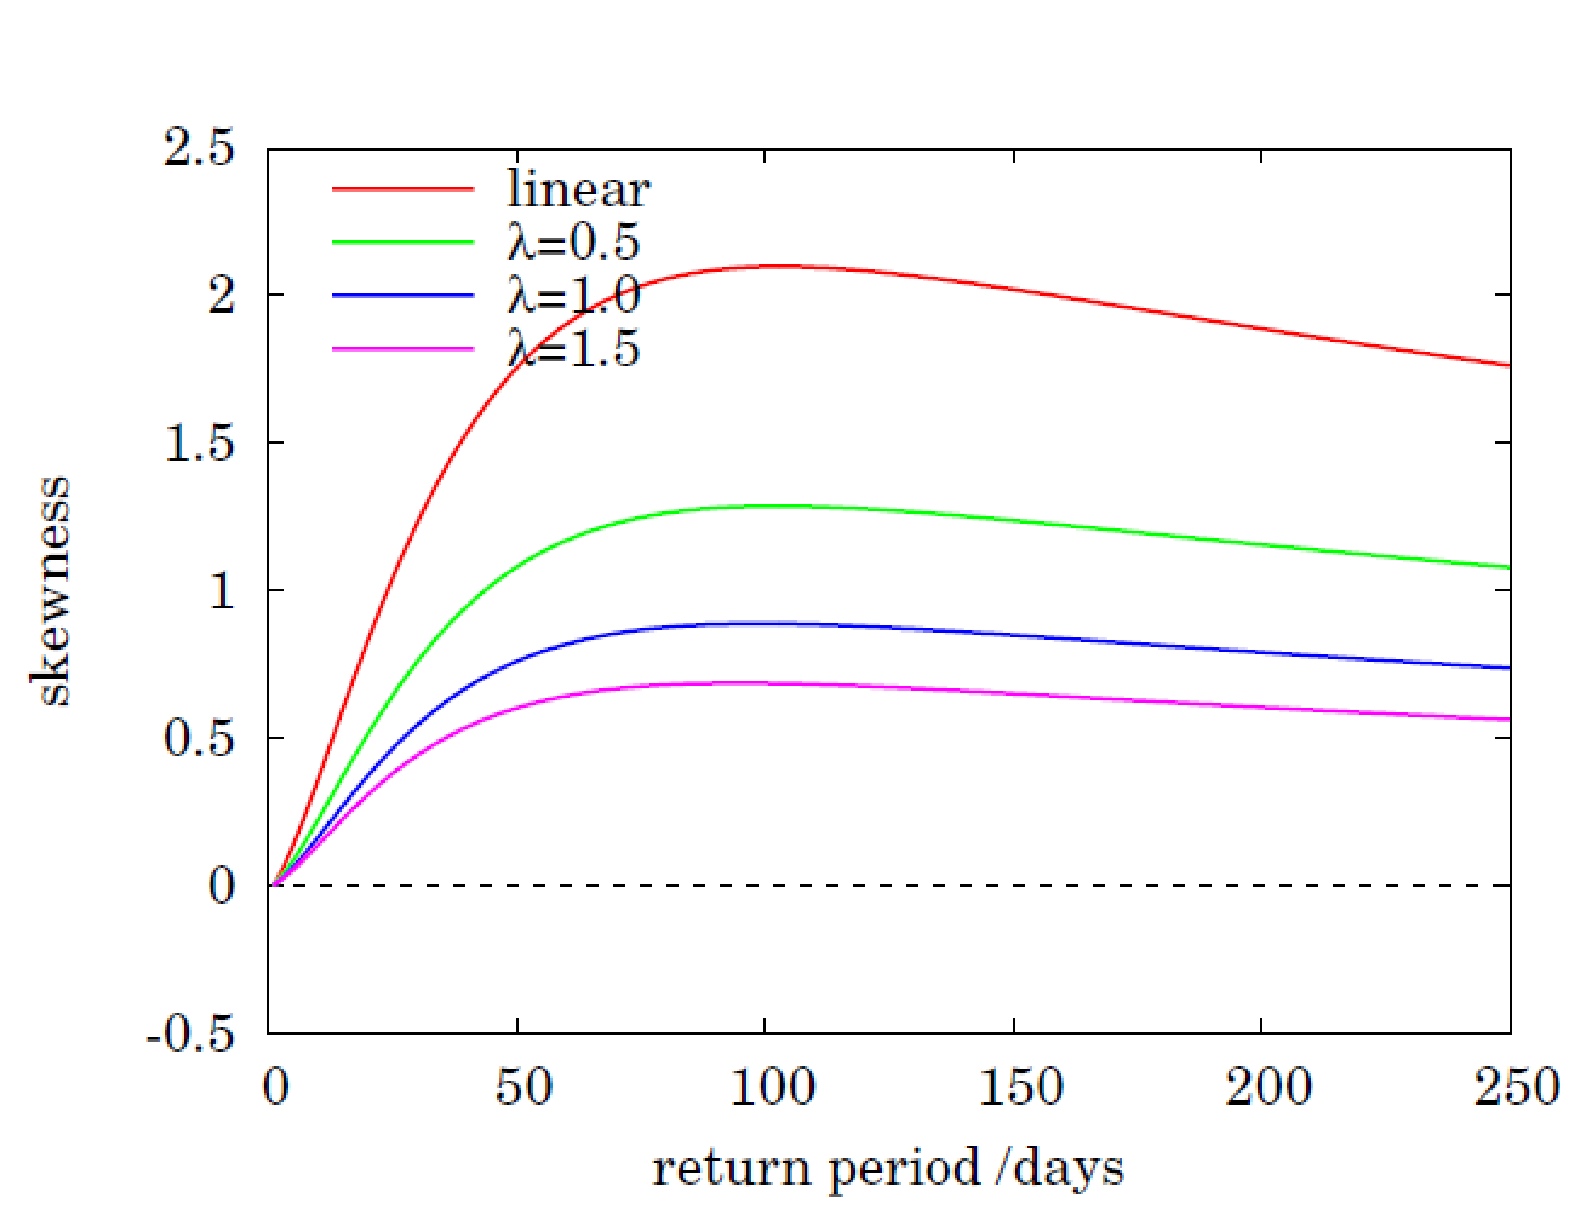
\includegraphics[scale=0.15]{docs/figures/L5/sigmoid_skewness.png}
    \caption{Sigmoid Skewness - peak closer in lowers it}
    \label{fig:enter-label3}
\end{figure}


\end{frame}

% \begin{frame}{Skewness and Nonlinear Transforms}
% \begin{figure}
%     \centering
%     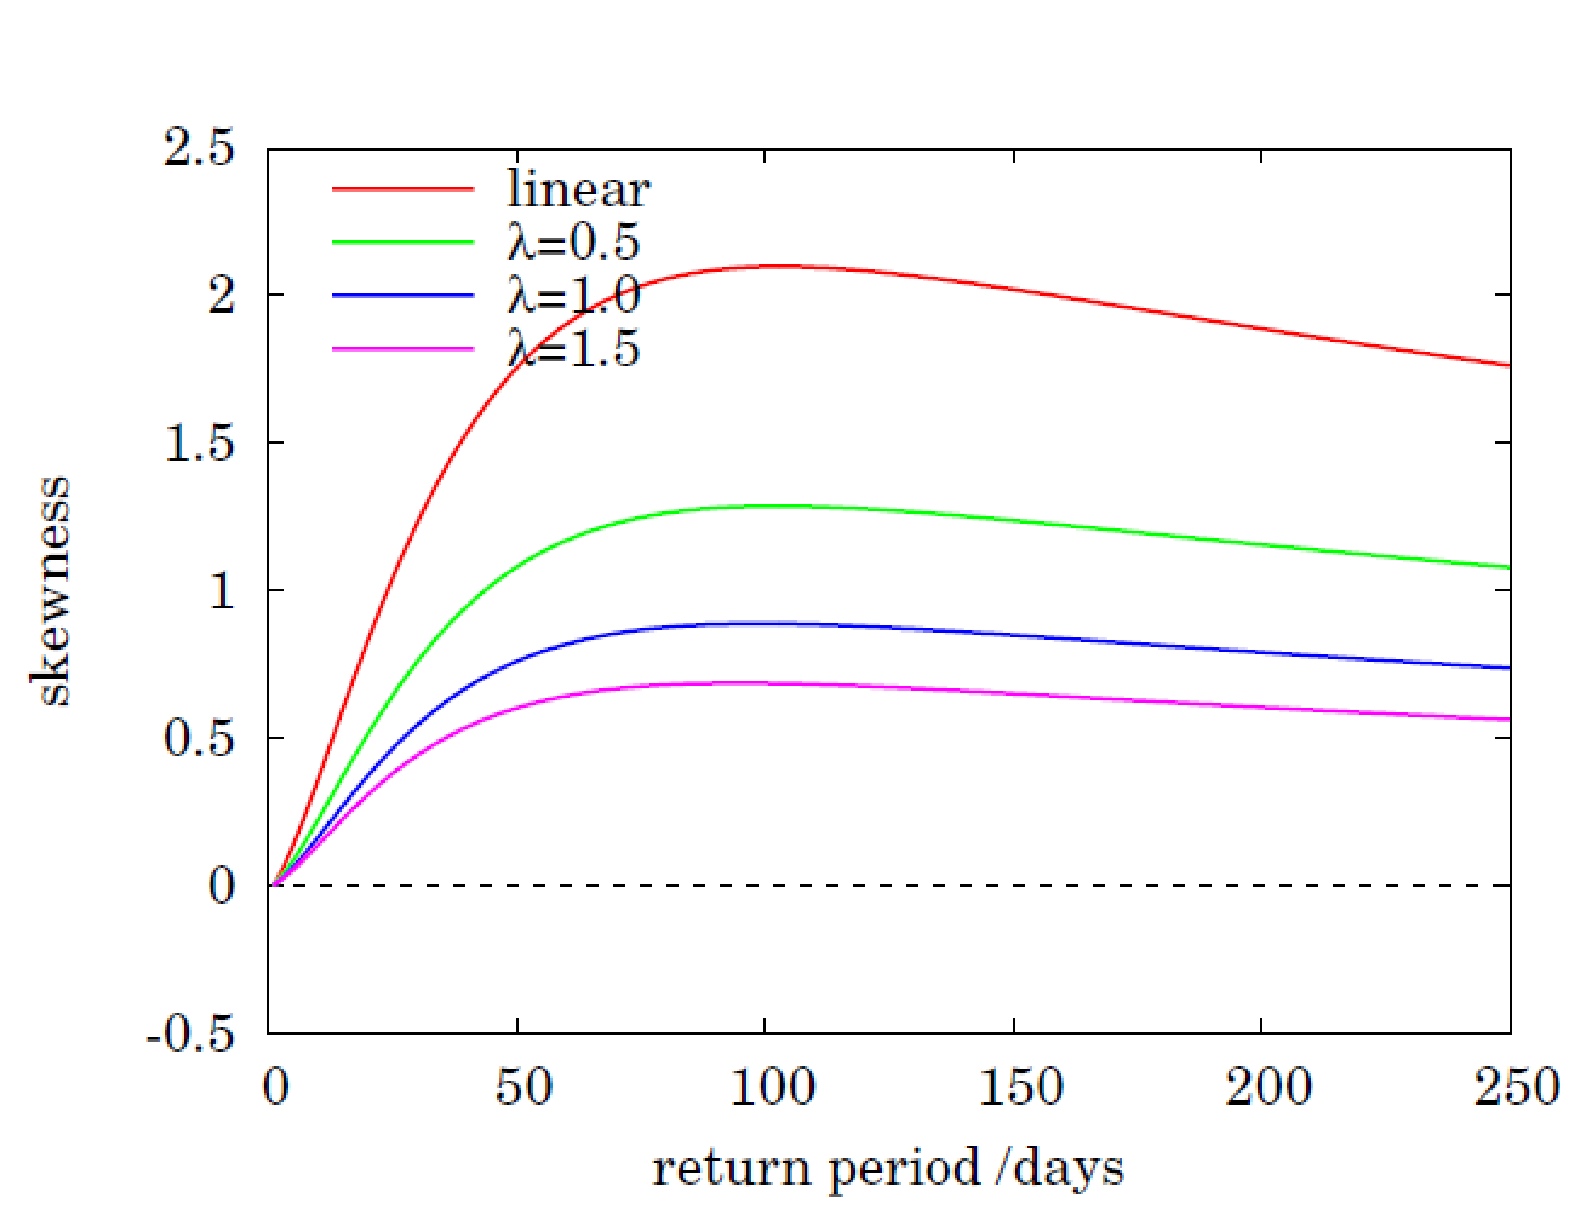
\includegraphics[scale=0.15]{docs/figures/L5/sigmoid_skewness.png}
%     \caption{Sigmoid Skewness - peak closer in lowers it}
%     \label{fig:enter-label}
% \end{figure}

% \end{frame}

\begin{frame}{Skewness and Nonlinear Transforms}
\begin{figure}
    \centering
    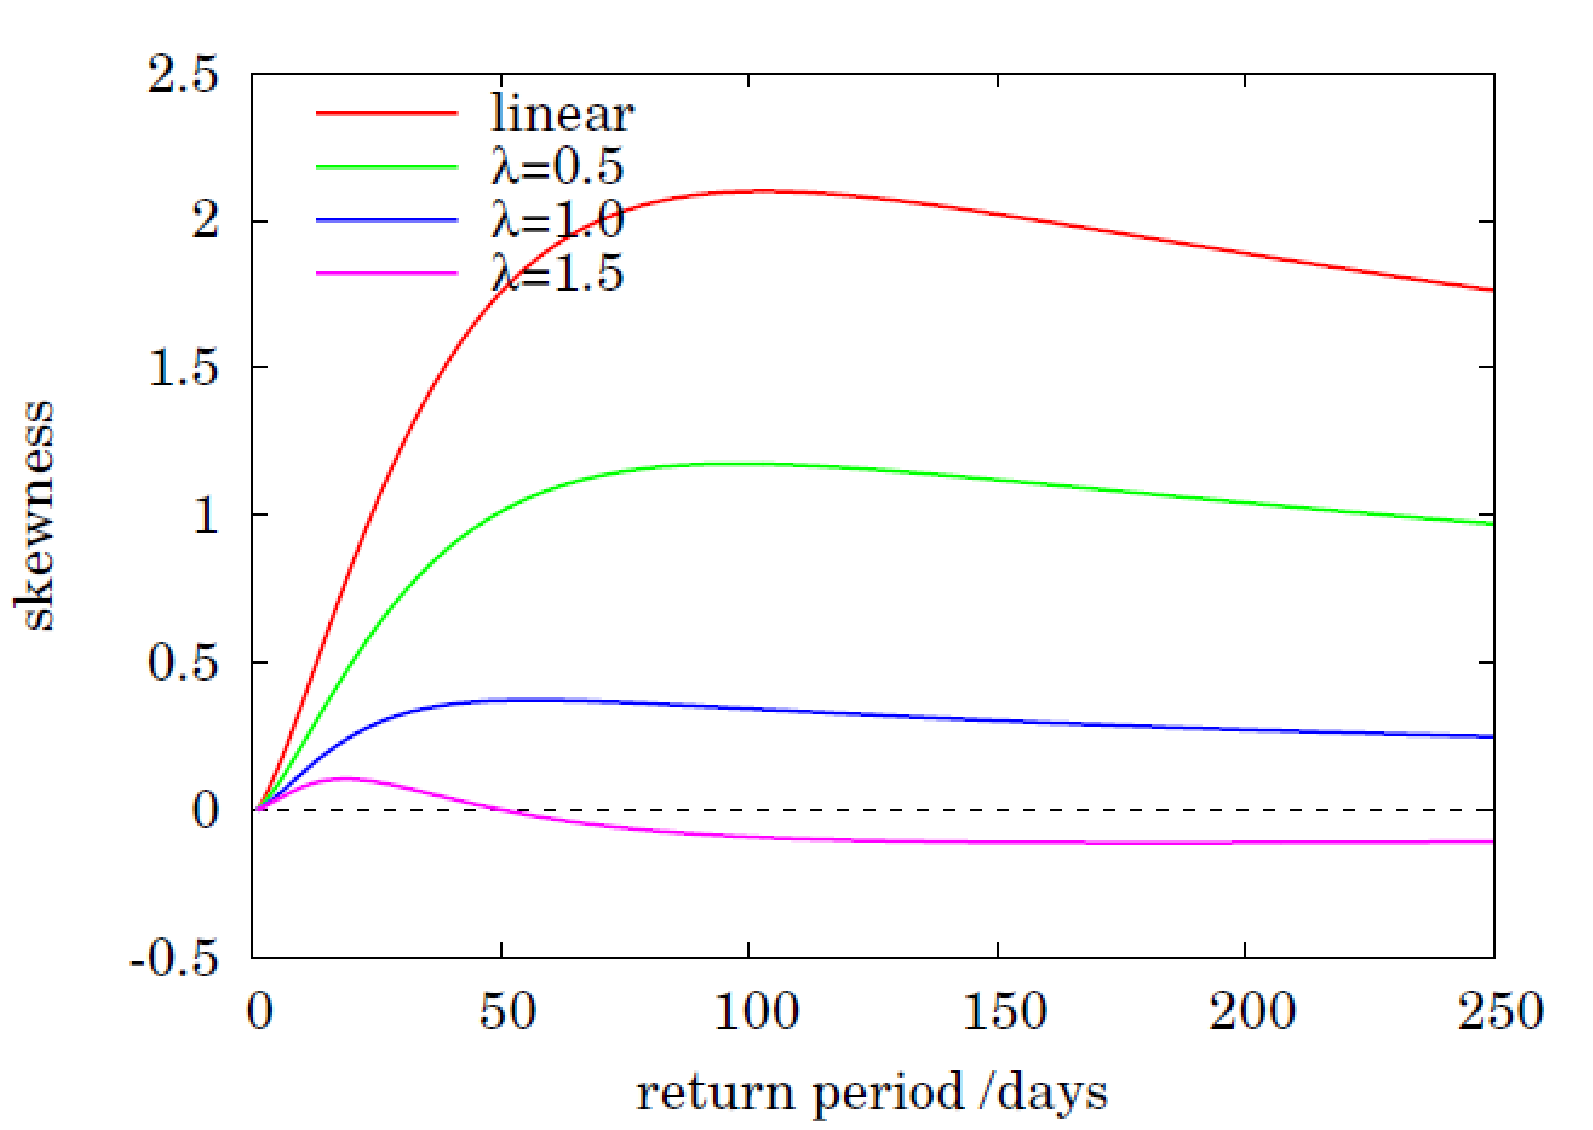
\includegraphics[scale=0.15]{docs/figures/L5/reverse_sigmoid_skewness.png}
    \caption{Reverse Sigmoid Skewness - peak closer/falls quicker in lowers it}
    \label{fig:enter-label4}
\end{figure}

\end{frame}






\section{Momentum and Responsiveness}
%%%%%%%%%%%%%%%%%%%
\begin{frame}{Responsiveness}
    \begin{itemize}
    \item 
    Short-term MA  - 
    \begin{itemize}
     \item more responsive - captures established trends near their start 
      \item higher transaction costs - bleeds away in a sideways market
    \end{itemize}
    \item 
    Long-term MA 
    \begin{itemize}
        \item less responsive - lagged response to new turning points  
        \item lower transaction costs - doesn't lose money in a sideways market
    \end{itemize} 
    \end{itemize}
\end{frame}

\begin{frame}{Trend via SDEs}

\begin{alertblock}{Trend via SDE}
\begin{itemize}
    \item Consider a nonlinear allocation depending on levels $\theta_t=f(S_t)$
    \item The total PnL is then $dV_t = f(S_t)dS_t$.
    \item Let $F(S) = \int_c^S f(s)ds$, then, if $S$ is deterministic
    \begin{align*}
        V(T)-V(0) &= \int_0^T f(S_t)dS_t\\
                  & = F(S_T) -F(S_0)
    \end{align*}
    \item If $S$ is stochastic, $dS=\mu_t S_t dt + \sigma_t S_t dW$ by Ito, we have
    $$
    V(T) - V(0) = \underbrace{F(S_T)-F(S_0)}_\text{option profile} 
    - \underbrace{\frac{1}{2}\int_0^T f'(S_t)S_t^2\sigma_t^2 dt}_\text{trading impact}
    $$
        
    
\end{itemize}


\end{alertblock}
\end{frame}


\begin{frame}{Trend via SDEs}

\begin{alertblock}{Trend via SDE}


We let 
    $$\frac{dS_t}{S_t} = \mu_t dt + \sigma_t dW$$
and define
$$d \hat{\mu}_t = -\lambda \hat{\mu }_tdt +\lambda \frac{dS_t}{S_t}$$

$\hat{\mu}$ is an EWMA, i.e. 
$$\hat{\mu}_t=\int_{-\infty}^t e^{-\lambda(t-s)}\frac{dS_s}{S_s}$$

Note that we still cannot represent all ARMA processes using SDE. Only MA terms. 
% AR terms requires integrodifferential SDE or functional SDE. Sometimes studied in physics or engineering literature. 
If we consider the trend following strategy using a single EWMA:

$$\frac{dV_t}{V_t} = m\frac{\hat{\mu}_t}{\sigma^2}\frac{dS_t}{S_t} $$ 


\end{alertblock}
\end{frame}


\begin{frame}{SDE approach}
\begin{alertblock}{SDE approach Cont'd}
Then we have the following identity (just using Ito's Lemma)



$$\ln(\frac{V(T)}{V(0)}) = \underbrace{\frac{m}{2\lambda}(\hat{\mu}_{T}^2-\hat{\mu}_{0}^2 )}_\text{option profile} + \underbrace{m\sigma^2 \int_{0}^T\bigl(\frac{\hat{\mu}^2}{\sigma^2}(1-\frac{m\sigma^2}{2}) - \frac{\lambda}{2}\bigr)  \, dt}_\text{trading impact} $$

\begin{itemize}
    \item {\bf Option profile} evolves quickly, lower bound of $-\frac{m}{2\lambda}\hat{\mu}^2_0$, and thus is more exposed to risky asset  if the initial trend is high (at the start).
    \item {\bf Trading impact} cumulative, evolves slowly. $m\ll 1$ then there is a positive contribution whenever $$|SR|> \sqrt{\frac{\lambda}{2}}$$
\end{itemize}
\end{alertblock}
\end{frame}

\begin{frame}{SDE approach}
\begin{alertblock}{SDE approach Cont'd}
A few sources that specifically use the SDE approach:
\begin{itemize}
    \item \href{https://papers.ssrn.com/sol3/papers.cfm?abstract_id=2465623}{Bruder-Gaussel: Risk-Return Analysis of Dynamic Investment Strategies}
    \item \href{http://thierry-roncalli.com/download/Momentum_Risk_Premium.pdf  }{Jusselin et al: Understanding the Momentum  Risk Premium}
    \item \href{http://www.thierry-roncalli.com/download/Alternative_Risk_Premia.pdf}{Hamdan et al: Alternative Risk Premia}

\end{itemize}
\end{alertblock}
\end{frame}



\section{Cross-Sectional Momentum}
\begin{frame}{Cross-Sectional}
\begin{alertblock}{Cross-Sectional Momentum}
\begin{itemize}
    \item We will cover this in some detail later on in factor investing.
    \item Cross Sectional Momentum: Buy the winners, sell the losers. 
    \item Carhart, \href{https://onlinelibrary.wiley.com/doi/10.1111/j.1540-6261.1997.tb03808.x}{On Persistence of Mutual Fund Performance}  was the first to introduce into Equities 
    \item Usually 12-month (less final month) momentum, ranking equities. Go long top-decile, short bottom-decile. 
    \item It is one of the most significant Equities factors
    \item Arguably, this is one of many methods for forming a portfolio.
\end{itemize}
    
\end{alertblock}
    
\end{frame}


\begin{frame}{Cross-Sectional vs Time-Series}
\begin{alertblock}{Cross-Sectional vs Time-Series}
\begin{itemize}
    \item Continued work on relationship.
    \item Some indication that Time-Series momentum works better. 
    \item Time-series is only concerned with winners when they are outperforming or losers when they are underperforming 
    \item Cross-sectional is concerned with relative performance. Digs deeper, including some stocks that may not be doing well in absolute terms
    \item Time-Series may be net-long or net-short as a consequence. Cross-sectional can be market-neutral.
    \item This is an active area of research.
\end{itemize}
    
\end{alertblock}
    
\end{frame}



\begin{frame}{Ranking in Portfolios}
\begin{alertblock}{Cross-Sectional Momentum and Ranking Portfolios}
\begin{itemize}
    \item Long the top decile and short the bottom decile, cash neutral is just one possible portfolio.
    \item There is an entire topic on portfolios from sorts.  
    \item Almgren-Chriss, \href{https://papers.ssrn.com/sol3/papers.cfm?abstract_id=720041}{Portfolios from Sorts}
    \item Nguyen-Lo \href{https://www.sciencedirect.com/science/article/pii/S0377221712002329?casa_token=JvNMb5IlRD4AAAAA:mucm7PNlGMnEvDQV02s8e-3h3lLqYrmbF2ET-YGWBKtah7KKMcZWvfHGakIHo-OVesjnW9bONQ4}{Robust ranking and portfolio optimization}
    \item Often the ranking of assets should have some difference.
    \item This is an active area of research.
\end{itemize}
    
\end{alertblock}
    
\end{frame}



\section{Other Topics in Momentum}

\section{Other Topics in Momentum}
\begin{frame}{Mean-Reversion, Momentum, Mean-Reversion}
\begin{alertblock}{Almost all assets seem to}
    \begin{itemize}
        \item Mean Revert over very short horizons (at various time-scales, intraday and over a few days)
        \item Trend over the medium Horizon
        \item Mean-revert (or have reversion to long-term value) over the very long-horizon
        \item Changes to this behaviour are possible. And certaintly breaks/break-outs/change-points are a profitable area,
        \item In general, if we keep the horizon the same each of these strategies can be profitable
    \end{itemize}
\end{alertblock}
\end{frame}

\begin{frame}{Mean-Reversion, Momentum, Mean-Reversion}
    \begin{figure}
        \centering
        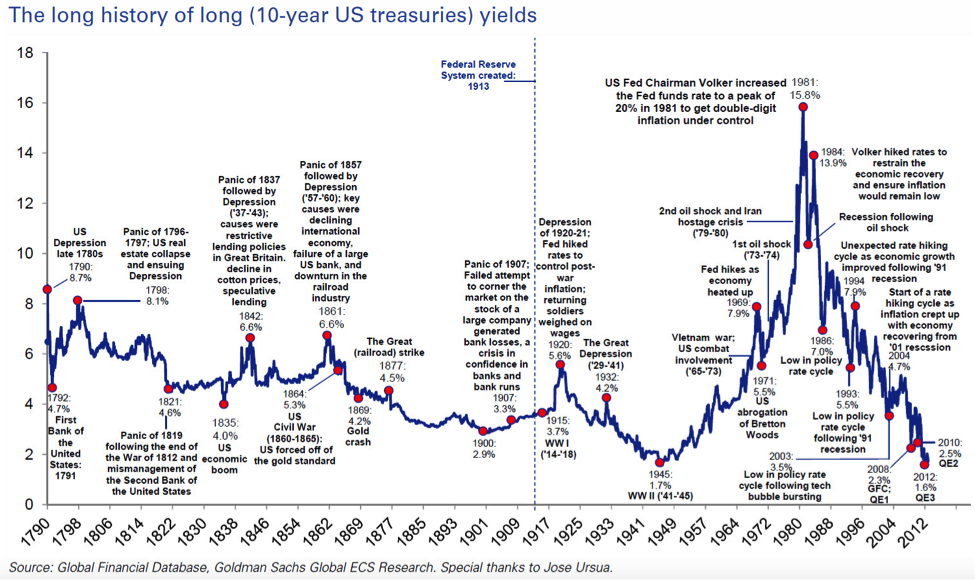
\includegraphics[scale=0.5]{docs/figures/History-of-Treasury-Yields.png}
        \caption{US Treasury Yields}
        \label{fig:enter-label}
    \end{figure}
\end{frame}


\begin{frame}{Momentum - Over Utilised?}
    \begin{alertblock}{Momentum Crowding}
        \begin{itemize}
            \item Momentum funds have grown rapidly over past 15 years.
            \item There is some cause to believe that returns are lower because of crowding
            \item In fact, Winton argued that some CTA AUMs were not CTA funds (from our first day's lecture) , primarily because this was a touchy point.
            \item Man AHL, recognising challenges, launched {\sl AHL Evolution} in 2006, to take advantage of momentum in {\sl less liquid} assets (funnily enough - $2^{nd}$ or longer utures contract, swap forwards, bonds etc) 
        \end{itemize}
    \end{alertblock}
\end{frame}

\section{An Exercise}

%%%%%%%%%%%%%%%%%%%%
\begin{frame}{Exercise}
\begin{alertblock}{Background - Momentum in Equities}
    \begin{itemize}
        \item Recall - Equities Indices typically trend in the medium term (e.g., 1y), but mean-revert in the short term (e.g., 10 days)
        \item Carhart recognised this and created the momentum factor sorting returns from 12m less the previous month.
        \item At that point buy the winners and hold. 
        \item It is also known that momentum stops  working after about 18m. Sometimes this is called mean-reversion even though the term is loose. (It is also unclear if we need to worry about this) 
    \end{itemize}
\end{alertblock}
\end{frame}

%%%%%%%%%%%%%%%%%%%%
\begin{frame}{Exercise}
\begin{alertblock}{Exercise - 1}
    \begin{itemize}
        \item Download an equities index  (e.g., SPX Index, SX5E Index, NKY, CAC, HSI etc) or futures series (CL1, CO1, NG1, GC1, C 1, etc), or ETF (SPDR, etc). At least 5 years.
        \item If a futures, make sure you account for the roll properly - 2-3 days before first notice date.
        \item Download an approx risk-free rate (SOFR - repo rate, or Fed Funds or SONIA or similar)
        \item Note: First Notice > First Delivery > Last Delivery $\approx$ Last Trade Date (Discussed in Futures section)
    \end{itemize}
\end{alertblock}
\end{frame}
%%%%%%%%%%%%%%%%%%%%
\begin{frame}{Exercise}
\begin{alertblock}{Exercise - 1b}
    \begin{itemize}
        
        \item Preferable to account for bid/ask, i.e., forecast and mark using 
        $$\hbox{mid}=\frac{\hbox{bid}+\hbox{ask}}{2}$$ 
        but enter and exit incurring costs 
        $$\hbox{tc} = \frac{\hbox{ask} - \hbox{bid}}{2}$$
    \end{itemize}
\end{alertblock}
\end{frame}

%%%%%%%%%%%%%%%%%%%%
\begin{frame}{Exercise-2}
\begin{alertblock}{Excercise - 2}
    \begin{itemize}
        \item Create an appropriate momentum signal given you know what you know.  
        \item Save at least 1y for testing
        \item "Train" by adapting for filter parameter(s) to ensure decent performance on the test set.
        \item By performance we mean Sharpe Ratio (Avg Excess Return/Stdev Returns). Do it by year and for entire train set. You can include \$ Returns or \% returns, etc. Adjust as you wish. Only when you are done, apply to test set.
        \item How have you accounted for what you know about the time-series?
        
    \end{itemize}
\end{alertblock}
\end{frame}


\section{References}
\begin{frame}{References}
\begin{alertblock}{Time-series and cross-sectional momentum}
    \begin{itemize}

 

    \item  Asness, Moskowitz and Pedersen, \href{https://pages.stern.nyu.edu/~lpederse/papers/ValMomEverywhere.pdf }{"Value and momentum everywhere." The Journal of Finance 68.3 (2013): 929-985.]} Momentum in all asset classes

  \item Moskowitz-Ooi-Pedersen, \href{http://papers.ssrn.com/sol3/papers.cfm?abstract_id=2089463}{ Time-Series Momentum}
   \item Lecture Notes \href{http://docs.lhpedersen.com/TSMOM_Slides.pdf}{Moskowitz' Lecture Notes}  Documents significant momentum in Equity index, currency, commodity, and bond futures for 58 instruments 
    \end{itemize}
\end{alertblock}
\end{frame}


\begin{frame}{References}
\begin{alertblock}{Varieties of Trend-following methods}
    \begin{itemize}

    \item Bruder, Zhao, Richard, Roncali,  \href{http://www.thierry-roncalli.com/download/lwp-tf.pdf }{Trend Filtering Mechanisms for Momentum Strategies} Practicalities of filtering - one method for trend-following 

    \item Moskowitz and Pedersen \href{http://papers.ssrn.com/sol3/papers.cfm?abstract_id=2603731}{Which trend is your friend? } Present a variety of different trend method, Many different methods can be used to construct basically the same signals


    \end{itemize}
\end{alertblock}
\end{frame}


\begin{frame}{References}
\begin{alertblock}{Other papers of note}
    \begin{itemize}
    \item Fung-Hsieh - first presented empirical paper on  straddle-like payoff   \href{https://www.trendfollowing.com/whitepaper/hsieh_fung_final_paper.pdf}{Fung Hsieh Risk in HF strategies}
    \begin{itemize}
    \item Some important empirical work on CTAs, showing the straddle-like payout.
    \item The theory is very facile (daily lookback straddles do *not* and *never did* exist). 
    \item The strategies are never perfectly efficient as would be true of the exotic lookback straddle.
    \end{itemize}
     \item Lo-Kaminski \href{http://papers.ssrn.com/sol3/papers.cfm?abstract_id=968338}{When do stop losses stop losses?}Also quite simple paper, Stop losses work only for trending series, hurt for mean-reverting

    \item Firoozye-Kohiyama \href{https://arxiv.org/abs/1905.05023}{Avoiding Backtest Overfitting} - Describes dynamic strategies including momentum and mean-reversion and 'optimal' ways of choosing how to weight them. 
    
    \end{itemize}
\end{alertblock}
\end{frame}


\section{What have we covered}
\begin{frame}{Learnings}
\begin{alertblock}{What we covered}
    \begin{itemize}
        \item Trading Strategies - Definitions
        \item Momentum, its history and pervasiveness
        \item Cross Sectional and Time-series Trend
        \item Momentum and Skewness
        \item Momentum's Responsiveness
        \item Futures, How to store them, how to roll them
        \item An Exercise in Momentum trading
    \end{itemize}
\end{alertblock}
\end{frame}




\end{document}
